\documentclass[12pt,a4paper,oneside]{report}
\usepackage{main}
%Begin Title
\title{
  {SIFT Object Detection in Ambiente Distribuito con Apache Hadoop}\\
  {\large Università degli Studi di Salerno}\\
  {
\includegraphics[width=5cm, height=5cm]{logo_standard.png}}
}
\author{Diego Avella, Angelo Passaro, Antonio Addeo}
\date{\today}
\begin{document}
  \maketitle
  %Begin Abstract
  \begin{abstract}
    Ci troviamo in una situazione storica, per quanto riguarda il mondo dell'informatica, dove enormi quantità di dati (nell'ordine dei terabyte o addirittura dei petabyte e in un  futuro non molto lontano di zettabyte) vengono processati. Questi dati devono subire analisi e trasformazioni in modo da poter essere utilizzati in settori che non riguardano solamente il mondo informatico: ambienti scientifici come l'ingegneria, la biologia, e la medicina sono i maggiori consumatori di queste informazioni e hanno bisogno di risolvere i loro "problemi" in modo semplice e il più velocemente possibile. Proprio per questo il calcolo parallelo in ambiente shared memory non è più grado di poter gestire e sostenere queste enormi moli di dati in input senza sorpassare con facilità i limiti di tempo (CPU) e di spazio (Ram e Disco) per poter rispettivamente calcolare i risultati e memorizzarli. La nascita del paradigma Map Reduce ideato da Google e del suo file system (GFS), reso famoso dalla Apache Foundation grazie rispettivamente alle implementazioni di Hadoop e HDFS, ha risolto una grandissima branca di problemi disparati senza dover ricorrere a soluzioni artificiose che tentano di ottimizzare a livelli estremi perdendo di portabilità ma che inoltre necessitano di dover essere continuamente aggiornate per poter andare incontro ai limiti fisici di cui si è parlato prima. L'obiettivo di questa tesi è quindi quello di dimostrare che un approccio distribuito di calcolo, attraverso il modello basato su Grid Computing, permette di "superare" questi limiti in maniera semplice e con risultati accettabili se non migliori che potenzialmente possono scalare con facilità. La tesina si propone di implementare un algoritmo parallelo di Object Detection tramite estrazione di caratteristiche utilizzando l'algoritmo SIFT di Lowe. Il primo capitolo tratterà delle basi su cui si fonda il calcolo distribuito e il Grid Computing, il secondo parlerà di come il framework Hadoop permette di programmare in ambiente distribuito tramite il paradigma Map-Reduce e infine si metteranno in pratica le conoscenze acquisite per implementare l'algoritmo, misurarne prestazioni, la potenziale scalabilità e infine ci saranno le conclusioni finali.
  \end{abstract}
  \tableofcontents
  %Start Thesis
  \chapter{Fondamenti di Calcolo Distribuito}
  In questo capitolo verranno introdotte le definizioni e i principi generali su cui si fonda il calcolo parallelo moderno. Verranno introdotti concetti fondamentali come granularità e parallelismo, si analizzeranno le infrastrutture di calcolo parallelo in ambiente distribuito più utilizzate ovvero Cloud Computing e Grid Computing e si presenteranno le limitazioni che il modello shared memory possiede rispetto al modello distribuito ripercorrendo la storia dell'informatica focalizzandoci sul destino che hanno subito le macchine parallele.
\section{Definizione di Calcolo Distribuito}
Il \textbf{Calcolo Distribuito} rappresenta un ramo dell'informatica che si occupa di studiare i \textbf{Sistemi Distribuiti}. Con quest'ultima definizione, facciamo riferimento ad un insieme di calcolatori che interagiscono tra loro (di solito tramite l'ausilio della rete) al fine di effettuare dei calcoli per concorrere ad un obiettivo comune che può essere un'erogazione di un servizio, il risultato di un algoritmo molto complesso etc. Un programma scritto per un ambiente distribuito è detto \textbf{software distribuito} e la programmazione distribuita è il processo di scrittura di questi software. Il protocollo con cui i calcolatori comunicano tra loro può essere di vario tipo come ad esempio HTTP, RPC, o basato su scambio di messsaggi. Il calcolo distribuito è nato sia grazie alla nascita di Internet, che ha permesso a macchine remote di comunicare tra loro, sia dovuto ad altre cause:
\begin{enumerate}
  \item \textbf{Il limite di potenza di calcolo da parte dei processori:} Se fino alla fine degli anni 90 l'incremento della frequenza di clock di un processore aumentava in maniera costante, permettendo così agli algoritmi sequenziali di migliorare le loro prestazioni ogniqualvolta usciva hardware migliore, con l'avvento delle architetture multicore si è raggiunto un limite difficilmente superabile.
  \item \textbf{L'enorme mole di dati da dover processare:} Da quando si è integrato l'ausilio dei computer anche in settori estranei all'informatica, gli addetti al mestiere si sono trovati a dover risolvere problemi che avevano come input enormi quantità di dati che non potevano nemmeno lontanamente entrare nella memoria di un unico computer oltre a non avere la potenza computazionale per poter restituire risultati in tempi umanamente accettabili. Se a questo aggiungiamo l'avvento dei Big Data e di tutte quelle branche di analisi dei dati che si sono diffuse a causa di quest'ultimo, possiamo tranquillamente affermare che risulta impossibile per un singolo computer poter processare il tutto. 
\end{enumerate}
\section{Granularità}
%TODO trattare meglio la granularità
La granularità rappresenta "l'intervallo che occorre a due processi per sincronizzarsi misurato in numero di instruzioni macchina"\cite{cattaneo88}. Da questa definizione possiamo sicuramente dedurre che la granularità è inversamente proporzionale ai dati su cui vogliamo operare: più il partizionamento dei dati è piccolo, più istruzioni saranno necessarie per sincronizzarsi e di conseguenza la granularità dei programmi sarà finissima, viceversa se i dati su cui operare è grande sono necessarie meno sincronizzazioni e quindi la granularità è più grossa (coarsed). Quello che offre, ad esempio, un'achitettura basata su Grid-Computing è quella di operare su una granularità più grossa al fine di poter usufruire al meglio dell'hardware di ogni singolo nodo sfruttando la \textbf{data-locality} e sincronizzarsi quando è solo strettamente necessario.
\section{Parallelismo}
Il \textbf{parallelismo} rappresenta la capacità con cui è possibile eseguire del calcolo in parallelo. È una caratteristica che dipende strettamente dalla granularità ed entrambe permettono di classificare le architetture di calcolo tramite la tassonomia di Flynn:
\begin{description}
  \item[SISD:] La sigla sta per \textit{Single Instruction Single Data} e non è presente nessuna forma di parallelismo in quanto le operazioni sono svolte in maniera sequenziale basandosi sulla classica architettura di \textbf{Von Neumann}. Un limite di questa architettura è sicuramente quello della singola connessione tra processore e memoria che rappresenta un collo di bottiglia per le prestazioni.
  \item[SIMD:] La sigla sta per \textit{Single Instruction Multiple Data} e il parallelismo è ottenuto dal fatto che ci sono più CPU che processano più flussi di dati in parallelo;è molto utilizzata per il calcolo scientifico ed è stata l'architettura che ha caratterizzato le grandi macchine parallele come \textit{Cry} e \textit{Connection Machine}.
  \item[MISD:] La sigla sta per \textit{Multiple Instruction Single Data} e il parallelismo è dovuto al fatto che più processi o task lavorano su un unico flusso di dati.
  \item[MIMD:] La sigla sta per \textit{Multiple Instruction Multiple Data} e il parallelismo è dovuto al fatto che più processori lavorano su più flussi di dati ed è l'architettura su cui si basano i cluster moderni.
\end{description}
Se invece vediamo il parallelismo dal punto di vista del programmatore è possibile distinguere due paradigmi principali:
\begin{description}
  \item[Parallelismo Esplicito:]con questo tipo di approccio il programmatore deve esplicitamente tenere conto di come suddividere i task e decidere come e quando sincronizzare questi ultimi. I vantaggi che ne derivano sono sicuramente un maggior controllo da parte del programmatore di quale parti del codice sia necessario parallelizzare oltre ad essere più efficiente ma questo comporta come svantaggio un maggiore sforzo da parte sua nel progettare la soluzione al problema. Un esempio di parallelismo esplicito è quando si usano librerie come MPI.
  \item[Parallelismo Implicito:] con questo tipo di approccio il programmatore scrive implicitamente del codice parallelo senza che lui ne sia effettivamente consapevole in quanto c'è chi si occupa di farlo per lui (un compilatore, un framework, un middleware). Gli svantaggi sono una perdita di controllo da parte del programmatore sul proprio codice ma col vantaggio che può focalizzarsi sulla sua risoluzione aumentando di molto la produttività. Un esempio di approccio implicito è quando si usano framework come Hadoop o Spark.
\end{description}
\section{Modelli di Calcolo Distribuito}
Per parlare di Calcolo distribuito e di Sistemi distribuiti dobbiamo sicuramente tenere conto dell'infrastruttura sottostante che sorregge l'intero sistema affinchè possa funzionare al meglio. Ad oggi sono in uso tantissimo due tipologie di infrastrutture: \textbf{Cloud-Computing} e \textbf{Grid-Computing}.
\subsection{Cloud-Computing}
In un'architettura basata sul Cloud-Computing, le risorse informatiche, di qualunque tipo e non solo computazionali, vengono fornite all'utente quando richiesto. In un' infrastruttura come il Cloud i computer che erogano i servizi non è detto che siano situati sulla medesima rete locale (anzi è un caso raro) e questo comporta comunque un sovraccarico per quanto riguarda la comunicazione remota tra i vari nodi. Esistono diversi tipi di servizi che il Cloud Computing mette a disposizione:
\begin{description}
     \item[SaaS:] (Software as a Service) l'infrastruttura cloud mette a disposizione tutto il necessario per accedere ed usufruitre di un software installato su di una macchina remota.
     \item[Paas:] (Platform as a Service)l'infrastruttura cloud mette a disposizione una piattaforma su cui è possibile installare eseguibili, librerire, programmi ed è a carico dell'utente gestire tutto il sistema. Questa tipologia di servizio è molto famosa e messa a disposizione da grandi big come Amazon (AWS) e Microsoft (Azure).
     \item[Iaas:] (Infrastructure as a Service)l'infrastruttura cloud mette a disposizione dell'utente oltre alle risorse virtuali anche quelle hardware che si dovrà gestire. 
   \end{description}   
\begin{figure}[!ht]
  \begin{center}
    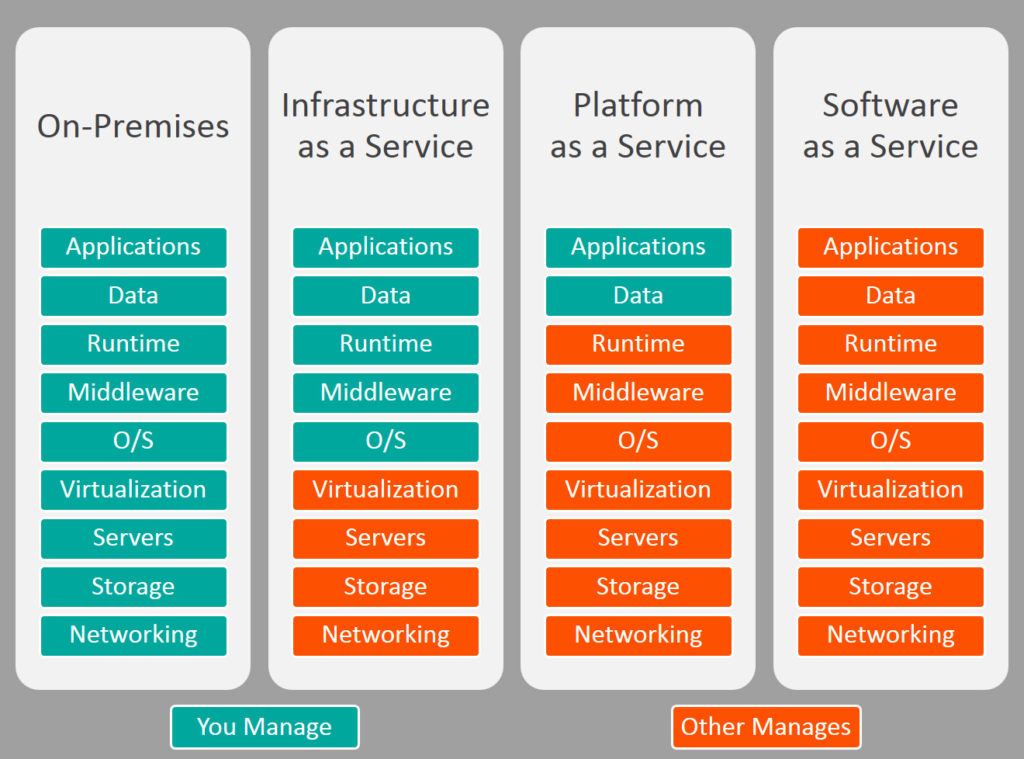
\includegraphics[width=\linewidth]{cloud.jpg}
    \caption{I Servizi Cloud}
    \label{fig:cloud}
  \end{center}
\end{figure}
\subsection{Grid-Computing}
In un'architettura basata sul Grid-Computing, le risorse informatiche(anche qui di qualunque tipo ma soprattuto di calcolo e memorizzazione) possono essere messe a disposizione dell'utente per risolvere determinati problemi (di solito di natura molto complessa dal punto di vista del tempo e dello spazio). La maggiore differenza con il Cloud la si evince su come è costruita l'infrastruttura dei nodi. I nodi come dice stesso la parola formano una specia di "griglia" ma in quest'ultima la rete che collega i vari nodi è formata da una rete locale e questo comporta un migliore aumento delle prestazioni a causa del basso consumo a livello comunicativo che i nodi devono effettuare per spedire i dati attraverso la rete. Questa infrastruttura è quella che viene comunemente chiamata \textbf{datacenter} e vari sono stati negli anni le possibili soluzioni architetturali che potessero permettere di aggiungengere nuovo hardware con facilità (quindi facilitare la scalabilità delle risorse), facili da gestire in fase di manutenzione e installazione del sistema operativo il tutto senza compromettere le prestazioni. 
\section{Modello Distribuito e Modello Shared Memory}
La domanda che ci si pone immediatamente è la seguente: Perchè eseguire calcoli in ambiente distribuito piuttosto che in shared memory? La risposta la si ottiene se si guarda indietro alla storia dell'informatica e del calcolo parallelo. I primi modelli di macchine parallele sono state ideate tra gli anni cinquanta e sessanta per poi raggiungere il loro periodo d'oro tra gli anni settanta e ottanta con l'avvento d macchine come Cry-1, Cry-2, Encore che avevano un enorme potenza oltre all'enorme quantità di denaro necessario per comprarle e manutenerle. Queste macchine ormai sono un ricordo lontano e la causa del loro fallimento è riconducibile a vari fattori:
\begin{description}
    \item [Fisico:] Come ci dice la "Legge" di Moore il numero di transistor all'interno di un processore raddoppia all'incira ogni 18 mesi. Sappiamo però che questo incremento non sarà, se non è già, più possibile perchè non si può ridurre la grandezza dei transistor oltre una certa soglia (14nm anche se sappiamo che Intel è riuscita ad arrivare fino ad 11nm) per non provocare problemi legati al \textbf{\textit{thermal noise}}. 
    \item [Sviluppo:] Aumentare il grado di multiprogrammazione tramite l'ausilio di thread ha sicuramente arginato in parte il problema ma non è sicuramente una soluzione in quanto i limiti imposti dalle architetture shared memory rappresentano comunque un collo di bottiglia che inficia sulle prestazioni. Per tentare di risolvere questo problema allora si è cercato di sfruttare modelli di calcolo parallelo tramite l'ausilio di standard di comunicazione (come ad esempio MPI) che sono una possibile soluzione ma rappresentano uno sforzo non da poco da parte del programmatore che deve esplicitamente decidere quali parti del proprio programma parallelizzare o meno.
    \item[Portabilità:] Macchine del genere avevano sistemi operativi dedicati ed era impossibile effettuare porting dei programmi paralleli su altri architetture dovuto anche alla grande quantità di famiglie di processori che, prima che Intel ed AMD conquistassero il mercato, esistevano e il passaggio ad architetture multicore peggiorò la situazione portando all'estinzione non soltando queste macchine ma anche un intera famiglia di sistemi operativi Unix-like
  \end{description}

  \chapter{Architettura di Calcolo Distribuito}
  \section{Datacenter}
Il \textbf{Datacenter} è una struttura composta da calcolatori che comunicano in rete, che aziende ed altre organizzazioni usano per organizzare, processare, memorizzare e disseminare enormi ammontare di dati. Essi rappresentano il cuore del business di un'organizzazione ed è necessario che soddisfino caratteristiche come scalabilità, sicurezza ed affidabilità oltre a possedere tutta l'attrezzatura necessaria come ad esempio la ventilazione, gruppi di continuità, sistemi di raffreddamento e naturalmente lo spazio necessario per installare il tutto. L'infrastruttura di un datacenter è cambiata molto durante gli anni e possiamo classificarla in tre categorie: 
\begin{description}
  \item[Infrastruttura Legacy:] In questa disposizione l'hardware è formato da tante commodity machines ma con l'obbligo di dover gestire ogni macchina separatamente ovvero si è costretti a dover installare su ogni macchina il sistema operativo, i programmi e le librerie necessarie. Da un primo impatto si può facilmente capire che con un numero molto grande di macchine la cosa risulta praticamente ingestibile e infatti questo modello è stato subito sostituito a favore delle architetture convergenti.
  \item[Infrastruttura Convergente:] In questa disposizione l'hardware è formato da enormi centri di calcolo che a differenza della struttura legacy sono gestiti tramite l'ausilio di un hypervisor quindi favorendo la gestione delle macchine ma con dei limiti dal punto di vista delle prestazioni in quanto la comunicazione con i dispositivi di memorizzazione avviene tramite una SAN\footnote{Storage Area Network} che rappresenta un collo di bottiglia nell'accedere e scrivere ai dati su disco.
  \item[Infrastruttura Iperconvergente:] Rappresenta la soluzione moderna per offrire un centro di calcolo performante. Questa architettura riprende il meglio delle due precedenti in quanto fa uso di commodity hardware, che costa poco, utilizza un hypervisor per gestire il datacenter ma la memorizzazione dei dati non avviene tramite una SAN. Quello che accade è che ogni rack possiede un insieme di piani che permette di aggiungere una motherboard formata da cpu, ram, e disco in modo che i dati delle singole motherboard possono accedere in maniera locale ai propri dischi aumentando le prestazioni e inoltre favorisce la scalabilità in quanto basta aggiungere al rack nuove motherboard quando è strettamente necessario.  
\end{description}
\begin{figure}[ht]
  \begin{center}
    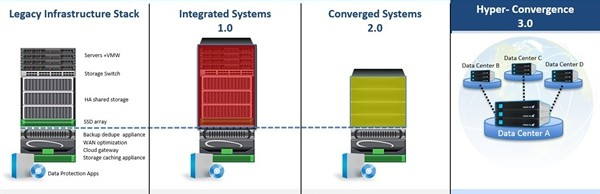
\includegraphics[width=\linewidth]{hyperconvergence.jpg}
    \caption{Le tre architetture}
    \label{hyp}
  \end{center}
\end{figure}
\section{Hypervisor}
Ogni commodity hardware che forma il moderno datacenter non si limita all'esecuzione di un unico sistema operativo in quanto questo rappresenterebbe uno spreco di risorse di memoria e di CPU che possono essede dedicate per eseguire altro calcolo. La virtualizzazione è stata la tecnologia fondamentale che ha permesso alle architetture dei datacenter di evolversi da legacy a convergenti. L'hypervisor rappresenta il componente software o hardware necessario per ottenere virtualizzazione e quando Bugnon nel 97 presentò Disco\cite{bugnon97} e il VMM (sta per virtual machine monitor ed è un sinonimo di hypervisor) nessuno avrebbe mai pensato che la sua intuizione lo avrebbe portato al successo fondando VMware.
\section{Gestione dello storage}
Essendo che un datacenter deve processare e memorizzare ordini di petabyte, quindi che non entrano in un disco commerciale, è stato necessario trovare delle soluzioni adeguate. La storia ci insegna che inizialmente i dati venivano memorizzati in enormi dischi rigidi (ricordiamo ad esempio SLED di IBM) che non solo costavano tantissimo ma occupavano tanto spazio con altezze che arrivavano addirittura a 14 pollici. La soluzione è arrivata nel 1988 grazie a Patterson e alla sua architettura \textbf{RAID} che ha evidenziato con i suoi esperimenti\cite{patterson88} che è possibile ottenere, mettendo insieme un array di dischi economici con appositi controller, più memoria, migliori prestazioni e tolleranza ai guasti.
\subsection{RAID}
L'acronimo sta per \textit{Redundant Array of Inexpensive Disks} e rappresenta l'innovazione che ha permesso di raggruppare diversi dischi dando la sensazione al sistema che possano essere utilizzati come se fossero un unico volume. L'implementazione del RAID può essere effettuata o hardware o software dove nel primo caso si usano controller hardware fatti a hoc molto costosi (più di tutti i dischi messi assieme), nel secondo caso il tutto viene gestito dal sistema operativo con un normale controller (che può essere SATA, ATI, SCSI, in fibra). Il tipo di array viene identificato dal livello RAID che determina il numero di dischi minimo necessario per poter essere configurato. La caratteristica fondamentale di questa tecnologia è quella della ridondanza che permette di individuare e correggere errori ed è ottenuta con differenti tecniche che variano a seconda del livello di RAID utilizzato:
\begin{description} 
  \item[RAID 0:]Questo livello non possiede ridondanza e utilizza lo \textbf{striping} (unità minima in cui viene diviso ogni file per la scrittura) per distribuire i file nei dischi facendo si che le letture e scritture avvengano in parallelo. Ha come svantaggio naturalmente la perdita totale dei dati in caso di rottura del disco.
  \item[RAID 1:]Questo livello fa sì che alcuni dischi vengano usati come copia per i dati in modo da intervenire in caso di guasto. Dal punto di vista delle prestazioni siamo pari a quelle di un singolo disco ma è presente la fault tolerance.
  \item[RAID 2:] Questo livello presenta delle caratteristiche simile al livello 1 ma con l'aggiunta di codici di correzione ECC dei dati. Questa configurazione è caduta in disuso a causa del fatto che ora i dischi attuali implementano di suo questa tipologia di correzione.
  \item[RAID 3:] Questo livello utilizza sia lo striping che il controllo della parità. Lo striping viene applicato a livello di segmenti e la parità mantiene le informazioni necessarie per poter recuperare i dati persi. In questo livello le scritture peggiorano poichè ad ogni scrittura si affianca il calcolo della parità e inolre la scrittura di essa avviene in un unico disco causando un collo di bottiglia sulle prestazioni totali.
  \item[RAID 4:] Questo livello utilizza le stesse funzionalità del livello 3 con la differenza che lo striping non viene effettuato con i segmenti ma a livello di blocchi.
  \item[RAID 5:] Questo livello utilizza le stesse funzionalità del livello 4 ma con la differenza che in questa configrazione non esiste un unico disco per la scrittura della parità ma su tutti vengono scritti dati o calcolo di parità (da notare che la parità non viene scritta sullo stesso disco dei dati). RAID 5 ha delle buone prestazioni che tendono a migliorare con l'aumento dei dischi installati.
  \item[RAID 6:] Questo livello ha le medesime caratteristiche del livello 5 con la differenza che effettua un doppio calcolo della parità (tramite codici di Solomon). Le prestazioni sono le medesime di RAID 5 con la presenza di una ridondanza aggiuntiva dei dati di controllo a causa della parità.
  \item[RAID Annidati:] Sono combinazioni di configurazioni di RAID permettendo così di accorpare le caratteristiche dei livelli. Le due combinazioni più diffuse sono la 01 e la 10. La prima prende due configurazioni RAID 0 e le combina in un RAID 1 e questo comporta che ogni gruppo di dischi conterrà la copia speculare dell'altro gruppo. Il secondo prende gruppi di dischi in RAID 1 e si combinano in RAID 0 permettendo così di vedere il tutto come se fosse un unico disco e inoltre permette la tolleranza del guasto di sue dischi.
\end{description}
\subsection{Software Defined Storage}
Ceph è una piattaforma di storage distribuito creata da Red Hat recentemente (2016) e rappresenta quella che potrebbe essere in futuro una valida alternativa a RAID per gestire la memorizzazione dei dati. Questa piattaforma fornisce intefacce di storage di diverse tipologie (a oggetti, a file) quindi permettendo una grande flessibilità ma soprattutto riesce a scalare nell'ordine degli exabyte. La replicazione dei dati avviene al livello software rendendo così Ceph una piattafroma indipendente dall'hardware. La ragione del suo successo risiede nel fatto che sia possibile accedere ai dati in maniera completamente trasparente e diversificata permettendo di adattarsi alle esigenze delle organizzazioni. Un'altra caratteristica a favore è che un sistema Ceph può essere costruito con commodity hardware riducendo di molto i costi a discapito di un controller RAID hardware. Ceph come molte altre realtà, rappresenta quello che oggi viene comunemente definito come \textit{Software Defined Storage} e nasce per andare incontro alle esigenze delle architetture iperconvergenti utilizzando la virtualizzazione per separare tutte le funzioni di storage dall'hardware.
\section{Sistema Operativo}
L'introduzione di tecniche efficienti per aumentare le prestazione dei dischi, non sono sufficienti per avere un datacenter efficiente. Anche il sistema operativo gioca la sua parte e deve essere implementato affinchè usi al meglio l'hardware sottostante. Questo aspetto non è da sottovalutare perchè il sistema operativo gestisce servizi cruciali come lo scheduling dei processi, gestione della memoria virtuale, mappatura dei blocchi liberi, etc... Durante la storia dell'informatica la sistemistica è stato un ambito di ricerca e sviluppo che ha sempre portanto ventate di novità questo grazie anche ad un ambiente universitario sempre competitivo e alla ricerca di nuove soluzioni che spalleggiassero la propria visione. Questo ha portato alla nascita di tantssimi sistemi, ognuno con delle caratteristiche particolari e che hanno gettato le basi per quelli moderni. Tra i più significativi è necessario citare:
\begin{description}
  \item[Tornado:] Tornado è stato uno dei primi sistemi operativi che scommise sul passaggio alle architetture multicore dei processori e si focalizzò tanissimo nello sfruttare al meglio questi ultimi massimizzandone le prestazioni sfruttando pincipi di località e tecniche di tipo Object Oriented.\cite{gamsa98}
  \item[SPIN:] SPIN è stato uno dei sistemi che ha visto nella programmazione ad oggetti un nuovo approccio per progettare sistemi operativi. Scritto completamente in un linguaggio ad alto livello come MODULA-3 vantava modularità, estensibilità senza compromettere di molto le prestazioni.\cite{bershad94}
  \item[System V:] L'unico sitema della famiglia Unix che è stato continuato ad essere sviluppato presso i laboratori AT\&T è usato tantissimo in ambito commerciale. Purtroppo il suo sviluppo è cessato nel 2003 a causa della schiacciante predominio di Windows, Linux, Mac.
  \item[BSD:] Ultimo vero superstite originario della famiglia Unix è stato uno dei primi sistemi ad includere il protocollo TCP/IP ed è famoso per la sua stabilità, affidabilità e rispetto per gli standard. In giro sono rimaste unicamente le sue controparti opensource ovvero FreeBSD e OpenBSD.
  \item[Windows NT:] Se MSDOS può non essere considerato un sistema operativo vero proprio, invece il suo successore Windows NT ha portato molti cambiamenti e Microsoft è stata una delle prime ad aggiungere il supporto ai processori Intel, in paticolare 386 e 486, intuendo da lì a poco che il mercato delle CPU si sarebbe pian piano ridotto ad un insieme ristretto di concorrenti. Questo unito alla sua semplicità ne hanno fatto il sistema operativo de facto utilizzato dall'utenza media.
  \item[Mac:] Anche Apple e Steve Jobs capirono presto che la nuova fetta di mercato su cui incentrare il nuovo business sarebbero stati i personal computer e c'era bisogno di un sistema operativo semplice ed estensibile. Codice Sorgente di BSD e il microkernel Mach messi assieme diedero vita a quello che oggi chiamiamo MacOS. Apple è stata una delle pochissime aziende big che credettero nello sviluppo di un microkernel e questa scelta le diede ragione però solo dopo tanti anni dal passaggio dai 32 ai 64 bit delle CPU.
  \item[Gnu/Linux:] Richard Stallman stanco della piega con cui il software proprietario stava prendendo piede decise di fondare il movimento Free-Software implementando insieme a decine di altri programmatori al mondo un sistema operativo che assomigliasse a Unix ma che fosse libero. Lo sforzo di tantissimi volontari diede luce al sistema GNU che non essendo ancora provvisto di un kernel (la loro scelta era di scrivere un microkernel ma la difficoltà nello sviluppo di quest'ultimo era molto alta) non gli permise di vedere la luce fino a quando un giovane studente finladese di nome Linus Torvalds non creò come tesi per il suo dottorato di ricerca un kernel monolitico che chiamò Linux. Fortuna volle che l'integrazione delle due parti fu molto semplice e anni di contributi da parte di tantissimi sviluppatori lo hanno reso il sistema operativo che oggi conosciamo: stabile, affidabile, robusto e praticamente compatibile con tipologia di hardware esistente. Queste sue caratteristiche lo rendono il signore incotrastato inambiente server e su piattaforma cloud.
\end{description}
Lo sviluppo però non fu solo dal punto di vista tecnico: anche dal punto vista algoritmico la scoperta di nuove soluzioni portarono al miglioramento dei sistemi operativi. Possiamo ricordare gli algoritmi di scheduling che sono stati progettati quanod computer e mainframe passarono ma monoutente a multiutente come ad esempio il \textbf{Fair-Scheduler} basato sul sistema a quotazioni e il \textbf{Lottery Scheduling} il cui funzionamento prevedeva un meccanismo simile al gioco della lotteria in cui l'utente col "biglietto vincente" poteva acquisire le risorse.
\subsection{Kernel}
Il componente fondamentale su cui si appoggia un sistema operativo è sicuramente il kernel. Esso si occupa dell'intera gestione dell'hardware fornendo dei meccanismi di base su cui si basano i servizi soprastanti del sistema. Proprio il numero di servizi di base che deve offrire il kernel è causa di un intero movimento che ha dato origine a vari approcci di tipo architetturale con cui deve essere sviluppato un kernel:
\begin{description}
  \item[Kernel Monolitico:] In un kernel di tipo monolitico, tutti i servizi del sistema operativo condividono la medesima area di memoria (ovvero tutto è all'interno del kernel space) del kernel ed eseguiti insieme ad esso. Il kernel espone i propri servizi tramite delle system call e permette un accesso performate all'hardware sottostante. Gli svantaggi possono essere di vario tipo: basta un unico errore in un modulo kernel per mandare in crash l'intero sistema, se il kernel comincia ad aumentare di dimensioni diventa troppo grande e soprattuto ingestibile da manutenere e soprattutto non sono portabili e quindi un passaggio potenziale ad una nuova architettura comporta la riscrittura di tutte le componenti.
  \item[Microkernel:] Il microkernel rappresenta come idea l'opposto di un kernel monolitico. L'idea alla base è di mantenere il kernel più piccolo possibile definendo unicamente le funzionalità fondamentali all'interno del kernel space (scheduling, gestione blocchi) e implementare all'interno dello user space gli altri servizi facendo sì che questi ultimi  interagiscano con il kernel attraverso scambio di messaggi tramite RPC. I vantaggi sono un kernel più compatto e più facile da manutenere, estendibilità ma al prezzo di un calo di prestazioni. C'è anche da sottolineare comunque che questo calo di prestazioni non è molto cospicuo come infatti hanno dimostrato gli studi su L4\cite{hartig97} e sui meccanismi di gestione della memoria virtuale\cite{rashid88,appel91}.
  \item[Kernel Ibridi:] Sono un ibrido tra un kernel monolitico e un microkernel e racchiudendo al suo interno qualche funzionalità in più di un normale microkernel.
  \item[Exokernel:] Sono un estremizzazione delle architetture kernel in cui il numero di astrazioni sull'hardware è ridotto all'osso permettendo agli sviluppatori di prendere le decisioni più appropriate e il kernel garantisce unicamente la gestione e messa in sicurezza delle risorse. Le applicazioni richiedono specifiche risorse fisiche (blocchi del disco, indirizzi di memoria) mentre il kernel assicura solo che le risorse siano disponibili e che l'applicativo abbia il diritto ad accederci.\cite{engler94}
\end{description}
\section{File System} 
In un datacenter è indispensabile avere un filesystem distribuito che sia trasparente e che nasconda all'utente che usufruisce del cluster l'effettiva locazione dei file sui dischi o di come siano memorizzati. L'informatica ha conosciuto diverse filosofie di implementazioni di filesystem su reti a partire dai primi anni 70 con l'invenzione del primo filesystem ma i primi tentativi concreti sono stati ottenuti con l'introduzione del protocollo \textbf{SMB} (Server Message Block) ed è ancora tuttora utilizzato da Windows e da Linux (Samba).
\subsection{AFS}
L'Andrew File system nato negli anni 80 è stato il precursore dei moderni file system distribuiti. Sviluppato alla Carnagie Mellow, presentava un architettura client server (Venus e Vice) e vennero sviluppati diversi protitipi. L'idea di base è che il client Venus richieda al server Vice solamente l'ubicazione del file quando è necessario aprire o chiudere quest'ultimo mentre invece per effettuare delle modifiche come ad esempio delle scritture vengono passate delle copie. Di AFS furono sviluppati vari prototipi tra per migliorarne le prestazioni e infatti nelle versioni successive furono introdotte comunicazione tramite RPC, um migliore meccanismo di gestione della cache e diminuiti i context switching dei processi Vice. Un difetto che ha portato questo file system ad essere poi lentamente rimpiazzato da NFS è stata una mancanza ottimale della gestione dellla coerenza dei dati in cache che non permetteva aggiornamenti in parallelo dei dati ma si era costretti a lavorare su copie dei dati e poi essere spedite nuovamente al server che, tramite meccanismi di callback, gestiva la coerenza.
\subsection{NFS}
Un aprroccio completamente ortogonale ad AFS fu il Network File System o conosciuto come NFS, ideato dalla Sun Microsystem nel 1984 di cui sono esistite 4 versioni, ognuna che introdusse nuove funzionalità. La maggiore differenza con AFS risiede nell'architettura con cui è costruito; mentre nel primo c'era una netta distinzione tra client e server, in NFS la comunicazione è sempre di questo tipo ma il componente che implementa il client e il server è il medesimo e questo ha permesso di aumentarne la portabilità, permettendo così di supportare piattaforme hardware e software eterogenee, e il modulo è caricato all'interno del kernel-space (a differenza di AFS dove sia client che server erano implementati nello user-space) avendo così un aumento delle prestazioni. Il funzionamento di NFS è molto semplice: Un file system (o una porzione di esso) viene montato su NFS facendo sì che diversi client accedano alle risorse (rispettando gli opportuni privilegi) e comunicando attraverso chiamate RPC.
\subsection{Coda}

\subsection{GFS}

  \chapter{Calcolo Distribuito con Hadoop e Map-Reduce}
  In questo capitolo si presenteranno i concetti e il funzionamento su cui si basa il framework Hadoop. Il capitolo si concentrerà inizialmente su una breve ricapitolazione della storia del framework, le sue origini e le cause del suo successo. Successivamente si analizzeranno nel dettaglio le sue componenti chiave ovvero HDFS e YARN e infine si introdurrà il modello Map Reduce spiegandone il funzionamento.
\section{Storia di Hadoop}
Il framework Hadoop fu creato da \textbf{Doug Cutting}, creatore di \textbf{Apache Lucene}, la libreria più utilizzata per quanto riguarda la ricerca di tipo testuale. Questo framework fonda le sue radici da \textbf{Apache Nutch}, una motore di ricerca per il web open source, a sua volta parte integrante del progetto Lucene. Scrivere un intero motore di ricerca da zero era un obiettivo molto ambizioso e il progetto Nutch partì nel 2002 ed ebbe un discreto successo tuttavia i creatori si resero immediatamente conto che la loro architettura non sarebbe stata in grado di scalare a sufficienza a causa dell'alto numero di pagine web da indicizzare (già allora ce ne erano più di un miliardo). Nel 2003 Google pubblicava il paper in cui introduceva il GFS e Nutch intuì che questo filesystem avrebbe risolto i problemi di memorizzazione e amministrazione dei dati che avevano e decisero di implementarne una versione open source che venne chiamata \textbf{NDFS} (Nutch Distributed File System). Un anno dopo Google pubblicò il paper che introdusse il paradigma Map-Reduce e ancora una volta il creatore capì che questa idea lo avrebbe aiutato a risolvere i problemi di Apache Nutch e nel 2005 il suo team implementò una sua versione open source e nel giro di 6 mesi tutti gli algoritmi del motore di ricerca furono adattati per essere eseguiti su NDFS e usando Map-Reduce. Questa "accoppiata" ebbe così tanto successo che nel Febbraio 2006, Nutch decise di spostarlo in un progetto indipendente chiamato Hadoop e nello stesso periodo Doug Cutting si unì a Yahoo! che forni un team dedicato e risorse finanziarie per trasformare Hadoop in un sistema che potesse essere eseguito per scalare anche sul web e ci riuscirono nel 2008 quando l'azienda annunciò che il suo indice di ricerca era stato generato da un cluster Hadopo da 10000 core. Nel Gennaio 2008 Hadoop divenne il progetto di punta della fondazione Apache ed è tuttora utilizzato da grandi compagnie come Facebook, New York Times e finanziato dai big dell'informatica come IBM, Microsoft e dalla stessa Google.
\section{Architettura di Hadoop}
Il passaggio dalla versione 1 alla versione 2 del framework ha portato enormi cambiamenti nella sua architettura e per evitare una descrizione troppo prolissa si introduce solamente la nuova architettura anche perchè è su quella che si basa questo lavoro. Le componenti fondamentali su cui si basa Hadoop sono le seguenti:
\begin{description}
  \item[Hadoop Common Module:] È il componente di base su cui si appoggiano tutti gli altri componenti del framework.
  \item[HDFS:] la sigla sta per "Hadoop Distributed File System" ed è il file system distribuito su cui si basa l'ecosistema Hadoop.
  \item[YARN:] Sta per "Yet Another Resource Negotiator" ed è il nuovo gestore delle risorse in Hadoop.
  \item[MapReduce:] È il componente di base che si occupa di implementare il paradigma lanciato da Google.
  \item[Altri Componenti:] Questi ultimi moduli rappresentano dei componenti che si poggiano su quelli elencati sopra.
\end{description}
\begin{figure}
  \begin{center}
    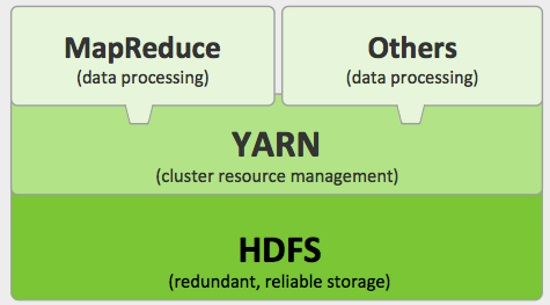
\includegraphics[width=\linewidth]{architecture.jpg}
    \caption{Architettura}
    \label{fig:architecture}
  \end{center}
\end{figure}
\subsection{HDFS}
HDFS è il filesystem distribuito che utilizza il framework Hadoop per processare i dati. I punti di forza su cui si basa sono i seguenti:
\begin{description}
  \item[Memorizzazione di grandi file:] Dove in questo contesto indichiamo file che sono centinaia di megabyte, gigabyte o terabyte.
  \item[Accesso dati:] HDFS è costruito intorno all'idea che il migiore pattern per processare i dati è "una scrittura e tante letture". Un dataset è tipicamente generato o copiato da una sorgente e successivamente varie analisi sono effettuate sul dataset nel tempo. Ogni analisi richiede grandi porzioni se non l'intero dataset quindi il tempo per leggere l'intero dataset è più importante della latenza di leggere il primo record.
  \item[Commodity Hardware:]Hadoop non richiede hardware costoso. È strutturato per essere eseguito su cluster basato su commodity hardware (hardware comunemente disponibile che può essere ottenuto da diversi fornitori).
\end{description}
\subsubsection{Blocchi}
Sappiamo che i dischi hanno una \textit{block-size} che rappresenta l'ammontare minimo di dati che possono leggere o scrivere. Di solito la grandezza di questi blocchi è nell'ordine dei kilobyte ma in HDFS questa grandezza è pari a 128MB e una caratteristica importante è che file più piccoli del blocco non occupano quest'ultimo interamente (ad esempio se avessimo un file da 1MB esso utilizzerà 1MB di disco e non 128). I motivi per cui questi blocchi sono così grandi sono vari: il primo è per minimizzare i tempi di ricerca nel disco, il secondo è che avere questa astrazione a blocchi, permette di memorizzare file più grandi di un singolo disco e inoltre semplifica la gestione della memorizzazione dei dati in quanto avere blocchi di taglia fissa permette di calcolare facilmente quanti ne possono essere memorizzati du di un disco ed elimina la gestione dei metadati (che vengono gestiti a parte).
\subsubsection{Namenode e Datanode}
Un cluster HDFS ha due tipologie di nodi che seguono il paradigma master-slave: un \textbf{namenode} (master) ed un numero di \textbf{datanode} (slave). Il primo gestisce il namespace del filesystem e i metadati per tutte le direcrory e i file e memorizza queste informazioni sul proprio disco locale oltre a conoscere la locazione dei blocchi di ogni file. I secondi invece memorizzano e processano i dati riportando periodicamente al namenode quale lista di blocchi memorizzano. La perdita del namenode comporta l'inutilizzabilità del filesystem ed è quindi importante avere un \textit{secondary-namenode} che periodicamente si sincronizza con il primary per fungere da backup in caso di guasti o malfunzionamento.
\subsection{Yarn}
\textbf{Apache YARN} (Yet Another Resource Negotiator) è il sistema della gestione delle risorse in Hadoop. Introdotto dalla versione 2 di Hadoop ha migliorato di molto le prestazioni del framework. Yarn fornisce i suoi servizi attraverso due processi manager, un \textit{resource-manager} (uno per cluster) per gestire l'uso delle risorse e un \textit{node-manager} che è eseguito su tutti i nodi nel cluster per lanciare e monitorare i container (Esegue i task con un insieme ristretto di risorse). Per eseguire un applicativo su YARN il client contatta il resource-manager e gli chiede di lanciare un \textit{application-master}. Quello che fa l'application master dipende dal tipo di applicazione: può semplicemente eseguire il job sul proprio container o richiederne altri per distribuire la computazione.
\begin{figure}
  \begin{center}
    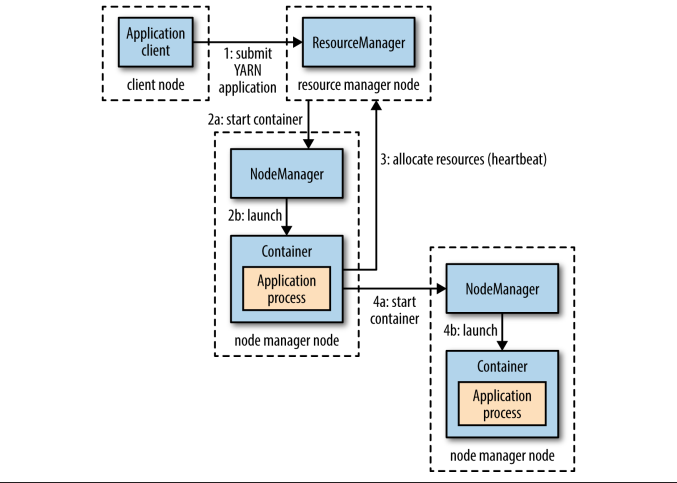
\includegraphics[width=\linewidth]{yarn.png}
    \caption{Esempio di Esecuzione di YARN}
    \label{fig:yarn}
  \end{center}
\end{figure}
\subsection{Paradigma Map-Reduce}
Map-Reduce è un modello di programmazione per processare i dati. I programmi Map-Reduce sono inerentemente paralleli, così da permettere di fare analisi di dati in larga scala se a disposizione di abbastanza macchine, in particolare questo modello funziona al meglio con dataset di grandi dimensioni. Hadoop è in grado di eseguire programmi Map-Reduce scritti in vari linguaggi tra cui Java, Python e Ruby e il suo funzionamento suddivide il lavoro in due fasi: la fase di map e di reduce. Ogni fase ha delle coppie chiave-valore come input e output, i cui tipi potrebbero essere scelti dal programmatore. Il programmatore specifica anche due funzioni: la funzione di map e la funzione di reduce. Nello specifico Map prende in input una coppia \textit{<K,V>} e restituisce in output una lista di coppie intermedie \textit{<K',V'>} mentre Reduce acquisisce in input una lista di coppie intermedie \textit{<K,V> } con la stessa chiave e restituisce in output una lista di coppie \textit{<K',V'>}. Il paradigma Map-Reduce fornisce oltre alle suddette funzioni, anche parallelizzazione, distribuzione automatica, fault tolerance, schedulazione I/O, status e monitoring. Un programma costruito secondo questo modello divide i dati in input tramite la libreria MapReduce ed eseguiti tramite varie istanze del programma su un cluster di macchine. Una delle istanze, il master assegna i task alle altre macchine, gli slave (o worker).
\subsubsection{Map}
In questa fase un worker legge il blocco di input assegnato, dopodiché estrae da esso le coppie \textit{<K,V>} e le passa una alla volta alla funzione \textit{map()}. La funzione \textit{map()} a sua volta produce delle coppie \textit{<K',V'>}. Per creare un mapper in Java è necessario che una classe estenda la classe Mapper che presenta la seguente firma:
\begin{lstlisting}
public class Mapper<KEYIN, VALUEIN, KEYOUT, VALUEOUT> {
  protected void map(KEYIN key, VALUEIN value, Context context) throws IOException, InterruptedException {
    //method body here
  }
}
\end{lstlisting}
Nel corpo del metodo \textit{map} è possibile inserire il proprio algoritmo per trasformare l'input nella maniera che si desidera da mandare al reduce con il metodo \textit{write} dell'instanza dell'oggetto di tipo \textit{Context}. Questo oggetto rappresenta il mezzo tramite il quale i Mapper e i Reducer interagiscono con il resto dell'ecosistema di Hadoop ed include informazioni fondamentali come ad esempio la configurazione dei job.
\subsubsection{Reduce}
Il master a questo punto assegna ad un worker un task di tipo reduce indicandogli una regione di dati da "ridurre". Un task reduce consiste nel prendere tutte le coppie \textit{<K,V>} raggruppate in modo che le chiavi siano uniche. Ogni gruppo viene passato quindi alla funzione \textit{reduce()}. In Java un reducer si crea estendendo la classe Reducer che ha la seguente firma:
\begin{lstlisting}
public class Reducer<KEYIN, VALUEIN, KEYOUT, VALUEOUT> {
  protected void reduce(KEYIN key, Iterable<VALUEIN> values, Context context) throws IOException, InterruptedException {
    //method body here
  }
}
\end{lstlisting}
Nel corpo del metodo \textit{reduce} è possibile inserire il proprio algoritmo per eseguire l'aggregazione degli output dei task map. Anche il reducer fa uso dell'oggetto \textit{Context} e del metodo \textit{write} per scrivere l'output prodotto. Sia Mapper che Reducer implementano due funzioni di hook chiamate all'inizio e alla fine di ogni task un'unica volta e sono rispettivamente il metodo \textit{setup()} e \textit{cleanup()} e sono utili quando c'è da effettuare un insieme di operazioni inizializzazione o di pulizia.
\subsubsection{Splitter}
Lo Splitter è quella componente che ha il compito di prendere l’intero input e di dividerlo in \textbf{InputSplit}, che verranno poi inviati ai vari map task. La mappatura \textit{< K, V >} degli InputSplit viene definita dalla classe InputFormat implementata. Hadoop mette a disposizione diverse implementazioni di InputFormat, ciononostante è possibile, ovviamente, definirne uno proprio da utilizzare durante la computazione implementando l’interfaccia \textit{InputFormat}. È da sottolineare il fatto che non si deve confondere l’InputSplit con il blocco utilizzato dall’HDFS. I due "blocchi" non necessariamente corrispondono. Possono infatti verificarsi dei casi in cui l’InputSplit utilizza dati presenti in più blocchi, causando un leggero overhead del sistema. Il framework Hadoop mette a disposizione diversi splitter oltre a poterni creare di nuovi creando una nuova classe che estenda la classe \textit{InputSplit}.
\begin{lstlisting}
public abstract class InputSplit {
  public abstract long getLength() throws IOException, InterruptedException;
  public abstract String[] getLocations() throws IOException, InterruptedException;
}
\end{lstlisting}
Questa classe non contiene alcun tipo di dato ma solo i riferimenti dell'ubicazione e della lunghezza di questi ultimi infatti questa classe è d'aiuto alle classi \textit{InputFormat} e \textit{RecordReader} le quali sono responsabili di recuperare e leggere i dati in maniera efficiente per i MapReduce Task.
\subsubsection{Partitioner}
I Partitioner sono responsabili di dividere le coppie \textit{<K, V>} intermedie generate dai MapTask ai vari Reducer per la funzione di Reduce. Per dividere in maniera equa i compiti ai Reducer, i partitioner usano una funzione di hash sulla chiave: $reducer = hash(K) \bmod n$. Implementare un partitioner personalizzato in Java richiede estendere la classe \textit{Partitioner} che presenta la seguente interfaccia:
\begin{lstlisting}
public abstract class Partitioner<KEY, VALUE> {
  public abstract int getPartition(KEY key, VALUE value, int numPartitions);
}
\end{lstlisting}
Di default hadoop utilizza un \textit{HashPartitioner} il cui funzionamento è stato riportato poc'anzi.
\subsubsection{Combiner}
I Combiner permettono l'aggregazione in locale prima della fasi di shuffle permettendo così di compattare l'input prima di essere spedito sulla rete ai reducer. In Java un Combiner deve estendere la classe Reducer, opera su ogni output del map task e le coppie chiavi-valore in output devono corrispondere a quelle del Reduce.
\subsubsection{Shuffle e Sort}
Map-Reduce garantisce che l'input ad ogni reducer sia ordinato per chiave. Il processo con il quale il sistema esegue il sort, e trasferisce gli output del map ai reducer come input, è conosciuto come shuffle.
\section{Come funziona un Job Map Reduce}
A grandi linee possiamo riassumere un'esecuzione di MapReduce nei seguenti punti:
\begin{enumerate}
  \item Lettura dei dati;
  \item Inputsplitting;
  \item Mapping;
  \item Combining; 
  \item Partitioning, Shuffling e Sorting;
  \item Reducing;
\end{enumerate}
È possibile eseguire un job MapReduce con una singola chiamata al metodo \textit{submit()} di un oggetto Job. Questa chiamata al metodo cela molta computazione ed è opportuno capire quali sono i passi compiuti da Hadoop  per eseguire un job. L'intero processo comprende, da una vista ad alto livello, cinque entità indipendenti:
\begin{enumerate}
  \item Il client, che sottomette il job MapReduce;
  \item Il resource maanger YARN, che coordina e monitora i container di calcolo sulle macchine del cluster;
  \item I node manager YARN, che lanciano e monitorano i container di calcolo sulle macchine del cluster;
  \item L'application master MapReduce, che coordina i task che eseguono il job MapReduce. L'application master e i task MapReduce sono eseguiti in container che sono schedulati dal resource manager e gestiti dai node manager;
  \item Il distributed filesystem (HDFS), che è usato per condivedere file tra altre entità.
\end{enumerate}
\begin{figure}
  \begin{center}
    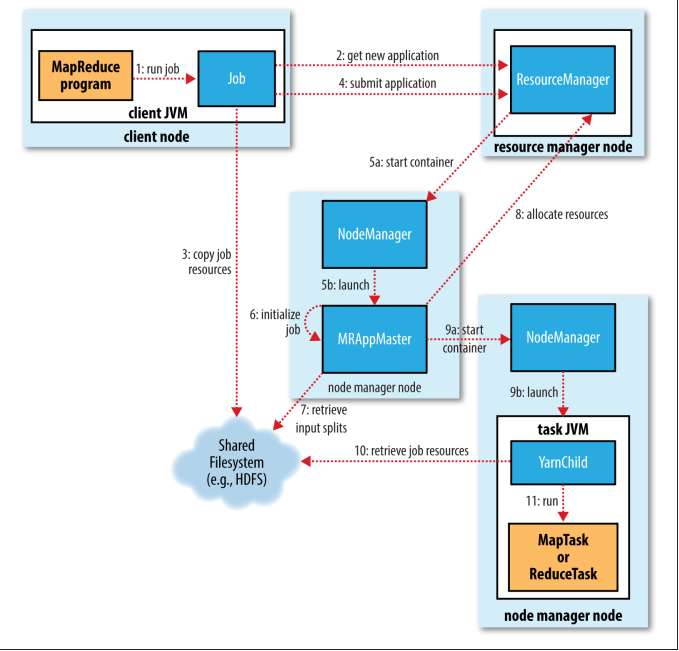
\includegraphics[width=\linewidth]{mapReduceJob.png}
    \caption{L'esecuzione di un job MapReduce di Hadoop}
    \label{fig:job}
  \end{center}
\end{figure}
\subsection{Sottomissione del Job}
Il metodo \textit{submit()}, effettuato su un Job, crea un'istanza interna JobSubmitter e chiama \textit{submitJobInterval()} su di esso. Avendo sottomesso il job, \textit{waitForCompletion()} sonda il progresso di job e riporta il progresso alla console se è cambiato dall'utlimo report. Quando un job è completato con successo, i risultati sono mostrati in output, altrimenti, l'errore che ha causato il fail del job è loggato in console.
\subsection{Inizializzazione del job}
Quando il resource maanger riceve una chiamata al metodo \textit{submitApplication()}, consegna la richiesta allo YARN scheduler. Lo scheduler alloca un container, e il resource manager lancia il processo dell'application master, sotto la gestione del node manager. L'application master per i job MapReduce è un'applicazione Java la cui classe principale è \textit{MRAppMaster}. Esso inizializza il job creando un numero di oggetti bookkeping per tenere traccia del progresso del job, dato che riceverà report sul progresso e sul completamento dai task. Successivamente, recupera gli input split calcolati nel client dal filesystem condiviso. Quindi crea un oggetto map task per ogni split, così come un numero di oggetti reduce task determinato dalla proprietà \textit{mapreduce.job.reduces}. I task a questo punto ricevono l'ID. L'application master deve anche decidere come eseguire i task che costituiscono il job MapReduce e se il job è piccolo, l'application master potrebbe scegliere di eseguire i task nella sua stessa JVM. Infine, prima che qualsiasi task venga eseguito, l'application master chiama il metodo \textit{setupJob()} sull'OutputCommitter. Per il FileOutputCommitter, che è di default, creerà la directory di output finale per il job e lo spazio di lavoro temporaneo per il task di output.
\subsection{Esecuzione del Task}
Una volta che a un task sono state assegnate risorse per un container su un particolare nodo dallo scheduler del resource manager, l'application master avvia il container contattando il node manager. Il task è eseguito da un'applicazione Java la cui main class è YarnChild. Prima che possa eseguire il task, localizza le risorse di cui il task ha bisogno, inclusa la configurazione del job e un JAR file, e qualsiasi file dalla cache distribuita. Alla fine, esegue il map o il reduce task. \\
Il YarnChild è eseguito in una JVM dedicata, così che qualsiasi bug nel map user-defined e le funzioni reduce (o anche in YarnChild) non influenzino il node manager, causandone il crash.\newline
Ogni task può eseguire azioni di setup e commit, che sono eseguite sulla stessa JVM come il task stesso e sono determinate dall'OutputCommitter per il job. Per i job file-based, il commit sposta l'output del task da una locazione temporanea alla sua locazione finale. Il protocollo di commit assicura che quando l'esecuzione speculativa è abilitata, solo di uno dei task duplicati verrà fatto il commit e gli altri saranno abortiti.
\subsection{Completamento di un job}
Quando il master application riceve una notifica che l'ultimo task per un job è completo, cambia lo stato per il job a "successful" e quindi, quando il Job sonda lo stato, apprende che il job è stato completato con successo e stampa un messaggio per dirlo all'utente e ritorna dal metodo \textit{waitForCompletion()}. Le statistiche e i counter di un Job sono stampati su console a questo punto. L'application master invia anche una job notification HTTP se è configurato per farlo. Questo può essere configurato dai client che vogliono ricevere callback, tramite la proprietà \textit{mapreduce.job.end-notification.url}. Infine, al completamento di un job, l'application master e i task container puliscono il loro working state (così l'output intermedio è cancellato), e il metodo \textit{commitJob()} di OutputCommitter è chiamato. Informazioni del Job sono registrate dal job history server per consentire successive interrogazioni dagli utenti se desiderato.
\subsection{Shuffle e Sort}
Lo shuffle è un'area del codebase dove raffinamenti e miglioramenti sono continuamente effettuati, costituisce il cuore di MapReduce ed è qui che avviene la "magia".
\subsubsection{Il lato Map}
Quando la funzione \textit{map} comincia a produrre output, questo non è semplicemente scritto su disco. Il processo è più complesso, e prende vantaggi dalla bufferizzazione delle scritture in memoria ed effettua qualche preordinamento per ragioni di efficienza. Ogni map task ha un buffer di memoria circolare su cui scrive l'output. Quando i contenuti del buffer raggiungono un certo limite di taglia, un thread in background comincerà a fare \textbf{spill} dei contenuti su disco, ovvero sposta i dati  dalla memoria RAM a quella del disco. I map output continueranno a essere scritti sul buffer fino a quando non avviene lo spill, ma se il buffer nel frattempo si riempie, il map si bloccherà sino al completamento dello spill. Gli spill sono scritti in round robin alle cartelle specificate dalla proprietà \textbf{mapreduce.cluster.local.dir}, in una sottocartella specifica al job. Prima che scriva sul disco, il thread prima divide i dati in partizioni corrispondenti ai reducer a cui saranno inviati alla fine e in ogni partizione, il thread in background esegue un ordinamento per chiave in memoria, e se c'è una funzione di combiner, è eseguito sull'output dell'ordinamento. L'esecuzione della funzione di combiner fa ottenere un map output più compatto, quindi ci sono meno dati da scrivere sul disco locale e da trasferire al reducer. Ogni volta che il buffer di memoria raggiunge il limite di spill, un nuovo spill file viene creato, così dopo che il map task ha scritto il suo ultimo record di output, ci potrebbero essere vari spill file. Prima che il task termini, si effettua il merge dei spill file in un singolo file di output partizionato ed ordinato. La proprietà di configurazione \textbf{mapreduce.task.io.sort.factor} controlla il massimo numero di stream di cui fare il merge alla volta; il valore di default è 10. Se ci sono almeno tre spill file, il combiner è eseguito di nuovo prima che il file di output sia scritto. I combiner potrebbero essere eseguiti ripetutamente sugli input senza influire sul risultato finale. Se ci sono solo uno o due spill, la riduzione potenziale nella taglia del map output non vale l'overhead dell'invocazione del combiner, quindi non è eseguita di nuovo per questo map output. È spesso una buona idea comprimere il map output alla scrittura sul disco, perchè fare ciò rende più veloce la scrittura su disco, risparmia spazio sul disco, e riduce la quantità di dati da trasferire al reducer. Di default, l'output non è compresso, ma è facile abilitare quest'impostazione settandola con \textbf{mapreduce.map.output.compress.codec}. Le partizioni del file di output sono rese disponibili ai reducer con HTTP. Il massimo numero di worker thread usato per servire le partizioni del file è controllato dalla proprietà \textbf{mapreduce.shuffle.max.threads}.
\subsubsection{Il lato Reduce} 
Il file di map output si trova sul disco locale della macchina che ha eseguito il map task (è da notare che nonostante i map output siano sempre scritti sul disco locale, i reduce output potrebbero non esserlo), ma ora è necessario per la macchina che sta per eseguire il reduce task per perchè ha bisogno del map output per la sua specifica partizione da vari map task nel cluster. I map task potrebbero finire in tempi diversi, quindi il reduce task comincia a copiare i loro output non appena ognuno è stato completato. Questa è conosciuta come fase di copia del reduce task. Il reduce task ha un piccolo numero di thread di copia così che possa prendere i map output in parallelo. Di default ci sono cinque thread, ma questo numero può essere cambiato settando la proprietà \textit{mapreduce.reduce.shuffle.parallelcopies}. Al completamento dei map task, essi notifcano il loro application master secondo il meccanismo di heartbeat. Perciò, per un dato job, l'application master conosce l'associazione tra i map output e gli host. Un thread nel reducer periodicamente chiede al master gli host del map output fino a quando non li ha recuperati tutti. Gli host cancellano i map output dal disco non appena il primo reducer li ha recuperati ma, siccome il reducer potrebbe successivamente fallire, aspettano fino a quando non gli viene detto di rimuoverli dall'application master, il che avviene dopo che il job è stato completato. I map output sono copiati nella memoria della JVM del reduce task se sono abbastanza piccoli (la taglia del buffer è controllata da \textit{mapreduce.reduce.shuffle.input.buffer.percent}, che specifica la proporzione dell'heap da usare per questo scopo); altrimenti, sono copiati su disco. Quando il buffer in memoria raggiunge il limite di taglia o raggiunge un numero limite di map output, ne viene effettuato il merge e lo spill su disco. Se un combiner è specificato, sarà eseguito durante il merge per ridurre la quantità di dati scritti su disco. All'accumularsi delle copie su dico, un thread in background ne fa il merge in file più grandi e ordinati così si risparmia tempo effettuando il merge in un secondo momento. Si nota che qualsiasi map output che è stato compresso (dal map task) deve essere decompresso in memoria per eseguire il loro merge. Quando tutti i map output sono stati copiati, il reduce task passa alla fase di ordinamento (che dovrebbe essere propriamente chiamata fase di merge, siccome l'ordinamento è stato effettuato nel lato map), che fa il merge dei map output, mantenendo il loro ordine di suddivisione. Ciò avviene in fasi: per esempio, se ci fossero 50 map output e il fattore di merge fosse 10, ci sarebbero cinque fasi dove ogni fase farebbe il merge di 10 file in 1, così alla fine ci sarebbero 5 file intermedi.
Piuttosto che avere una fase finale che fa il merge di questi cinque file in un unico file ordinato, il merge salva un trip su disco fornendo direttamente la funzione di reduce in quella che è l'ultima fase: la fase di reduce. Il merge finale può venire da un misto di segmenti in memoria e su disco. Il numero di file di cui si fa il merge in ogni fase è in verità più sottile di quanto quest'esempio suggerisca. Lo scopo è fare il merge del numero minimo di file da ricevere al fattore di merge per il passo finale. Quindi se ci fossero 40 file, il merge non farebbe il merge di 10 file in ognuna delle quattro fasi per ottenere 4 file. Invece, la prima fase farebbe il merge di solo 4 file, e le seguenti tre fasi farebbero il merge i 10 file. I 4 file ottenuti con il merge e i 6 file (di cui non è stato fatto ancora il merge) fanno un totale di 10 file per la fase finale.
\begin{figure}
  \begin{center}
    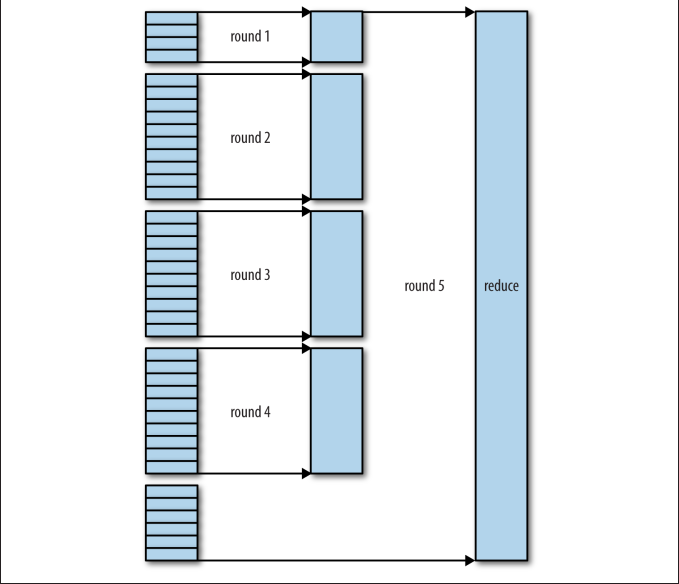
\includegraphics[width=\linewidth, scale=0.3]{effmerge.png}
    \caption{Merge efficiente per 40 segmenti di file con un fattore di merge pari a 10}
    \label{fig:merge}
  \end{center}
\end{figure}
Il numero di fasi rimane invariato; è solo un'ottimizzazione per minimizzare la quantità di dati scritti su disco, dato che il passo finale fa il merge direttamente nella reduce.
Durante la fase di reduce, la funzione di reduce è invocata per ogni chiave nell'output ordinato. L'output di questa fase è scritto direttamente sul filesystem di output, tipicamente HDFS. Nel caso di HDFS, dato che il node manager sta anche eseguendo un datanode, il primo blocco di replica sarà scritto sul disco locale.
\newpage
\section{Progetti Correlati}
la fondazione Apache ha creato un insieme di progetti che si appoggiano su Hadoop, tutti quanti di ottimo successo, e che si focalizzano su particolari casi d'uso:
\begin{description}
  \item[Apache Avro]:È un sistema di serializzazione dei dati utilizzato per poter sostituire quello che viene comunemente definito il problema maggiore di Haddop ovvero la non portabilità dei dati serializzati tramite i \textit{Writable}. I dati vengono descritti tramite l'ausilio di schemi scritti in JSON oppure tramite \textit{L'Avro IDL}. Un'altra caratteristica è che questi file possono essere splittabili e compressi e quindi utili per poter essere utilizzati dal MapReduce ed esendo indipendenti dal linguaggio, possono essere consumati anche utilizzando altri linguaggi di programmazione che non siano Java.
  \item[Apache Parquet:] È un formato di storage a colonne capace di memorizzare in maniera efficiente dati innestati. Memorizzare a colonne può essere molto vantaggioso in termini di spazio e di efficienza: nel primo caso lo storage è più efficiente di quello a righe perchè i dati sono "simili" e facili da codificare (ad esempio se si volesse memorizzare un timestamp si portebbe memorizzare il primo valore e nelle colonne succesive solamente i delta di tempo passati), nel secondo caso un query engine può saltare le colonne che non sono utili alla query. Questo formato è stato sviluppato da Twitter e Cloudera (uno dei piàù importanti fornitori di ambienti hadoop) utilizzanod tecninche innovative per memorizzare file in formato colonne rendendo minimi gli overhead. Anche questo fomrmato ècompatibile con MapReduce.
  \item[Apache Flume:] Ci sono molti sistemi che non fanno uso dell'HDFS per processare i dati ma allo stesso tempo hanno bisogno del MapReduce per processarli. Apache Flume cerca di andare incotro a questa esigenza, ed ha creato un ecosistema per processare enormi moli di dati event-based per poi mandarli ad Hadoop. Un esempio possono essere il log file di un web server e in questo caso Flume automatizza il processo di aggregazione dei file e spostamento sull'HDFS in maniera trasparente. L'idea è quella di lanciare dei processi Java (agent) in distribuito che collezionano i dati, li aggregano e li memorizzano nella sua destinazione finale.
  \item[Apache Sqoop:] A volte può succedere che il dataset su cui debba lavorare un job MapReduce, sia memorizzato in maniera struttrata all'interno di store strutturati come ad esempio un RDBMS. Sqoop risolve questo problema estraendo questi dati passandoli così ad Hadoop per effettuare le sue analisi.
  \item[Apache Pig:] Basato su MapReduce, si pone ad un livello di astrazione ancora più alto, permettendo di manipolare dati più complessi ed effettuando operazioni che non sono possibile normalmente su Hadoop (come ad esempio le join tra i dati). È formato da due componenti: il linguaggio utilizzato per lavorare sul flusso dei dati chiamato \textbf{Pig Latin} e l'ambiente di esecuzione che può essere centralizzato o distribuito al di sopra di un cluster Hadoop. È stato reato da Yahoo in risposta alle loro esigenze di effettuare mining su enrìormi moli di dati. 
  \item[Apache Hive:] È un framework sviluppato per effettuare data warehousing con Hadoop. Ideato da Facebook per permettere a chi ha una buona padroanza con SQL di eseguire query su enormi volumi di dati e ad oggi riscuote un buon successo perchè utilizzato da molte organizzazioni per scopi di tutti i tipi.
  \item[Apache Crunch:] È un insieme di API ad alto livello per produrre pipeline di MapReduce job. Il vantaggio principale che offre è che utilizza come tipi di dato quelli di Java, un insieme di operazioni di trasformazione dei dati già pronte all'utilizzo.
  \item[Apache Spark:] Anch'esso serve per processare moli di dati ma a differenza degli ambienti precedenti, non si appoggia su MapReduce ma utilizza un suo runtime  però può essere integrato con YARN e HDFS. Spark è conosciuto per la sua abilità di mantenere grossi dataset in memoria tra i diversi job e questo approccio funziona bene su algoritmi di tipo iterativo e su analisi interattive.
  \item[Apache HBase:] È un database distribuito orientato a colonne costruito al di sopra di HDFS. Il suo uso comune è per costruire \textbf{webtable}.
  \item[Apache Zookeeper:] È un servizio di coordinamento che permette di costruire applicazioni distribuite riducendo al minimo le failure.
\end{description}

  \chapter{Utilizzo di Hadoop per Object Detection }
  In questa capitolo si descriverà il problema affrontato per poi passare alle versioni sequenziale e distribuita della soluzione, e infine si discuterà delle prestazioni delle due versioni.
\newline
\section{Descrizione del problema}

Il problema affrontato in questo studio riguarda l' applicazione dell'algoritmo \textbf{SIFT}(Scale-Invariant Feature Transform) per effettuare object detection. L' object detection è una tecnologia informatica correlata alla visione artificiale e all'elaborazione di immagini che si occupa di rilevare istanze di oggetti semantici di una determinata classe in immagini e video digitali. Il rilevamento di oggetti ha applicazioni in molte aree della visione artificiale, tra cui il recupero di immagini e la videosorveglianza. 
Per ogni oggetto in un'immagine, ci sono molte features, che sono caratteristiche interessanti dell'oggetto, le quali possono essere estratte in modo da fornire una descrizione "caratteristica" dell'oggetto. Questa descrizione estratta da una immagine campione può poi essere utilizzata per identificare l'oggetto durante il tentativo di individuare l'oggetto in una immagine contenente più oggetti. Per poter recuperare queste features esistono diversi algoritmi quali per esempio SURF(Speeded Up Robust Features), ORB (Oriented FAST and Rotated BRIEF) e SIFT in questo studio ci siamo concentrati su quest'ultimo il quale è un algoritmo cpu-intensive e quindi ci interessava analizzare il suo comportamento in un ambiente distribuito.

\subsection{SIFT}
Scale-invariant feature transform (SIFT) è un algoritmo utilizzato in computer vision che permette di rilevare e descrivere caratteristiche pubblicato da David G. Lowe\site{lowe04} nel 2004.
L'algoritmo consiste in un metodo in grado di estrarre delle caratteristiche distintive invarianti da un immagine che possono essere utilizzate per effettuare un matching tra diversi oggetti. Le caratteristiche sono invarianti rispetto alla scala e alla rotazione dell'immagine e sono mostrate per fornire una robusta corrispondenza su una vasta gamma di distorsioni affini, cambiamenti nel punto di vista 3D, aggiunta di rumore e cambiamento nell'illuminazione. L'algoritmo esegue cinque step:
\begin{itemize}
\item \textbf{Scale-space Extrema Detection}
Per poter individuare dei keypoints abbiamo bisogno di diverse scale di un immagine quindi viene applicato un filtro per la scala. Questo filtro utilizza Laplaciana di una Gaussiana(LoG) che permette di rilevare blob di varie dimensioni grazie all'utilizzo $\sigma$ che funge come parametro di scala. Poichè LoG è costoso SIFT usa la differenza gaussiana(DoG) come alternativa che è una approssimazione del primo. La DoG è ottenuta come differenza di sfocatura gaussiana di un immagine con diversi $\sigma$ (si parte da un valore iniziale di $\sigma$ fino ad arrivare $k\sigma$) . Questo processo viene eseguito per diverse ottave dell'immagine.

\begin{figure}[!h]
	\begin{center}
    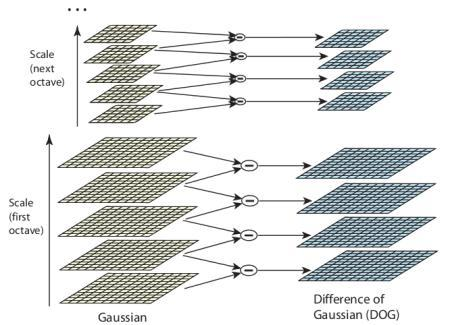
\includegraphics[scale=0.4]{DoG.jpg}
    \caption{Ottave di un immagine}
    \label{fig:DoG}
    	\end{center}
\end{figure}

Una volta trovato DoG vengono cercati i keypoints che rappresentano meglio l'immagine confrontando i pixel su diverse scale, per esempio un pixel in una immagine viene confrontato con i suoi 8 vicini e e con i 9 pixel della scala precedente e successiva.

\begin{figure}[!h]
  \begin{center}
    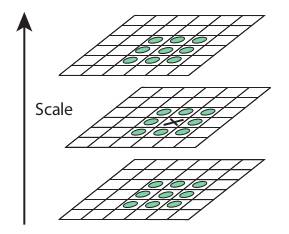
\includegraphics[scale=0.5]{kp.jpg}
    \caption{Ricerca di un keypoints}
    \label{fig:kp}
    	\end{center}
\end{figure}

%Il paper fornisce alcuni dati ottimali e sono: numero di ottave = 4, livelli di scala = 5 valore iniziale $\sigma$ = 1.6 e k = 2-$\sqrt$.

\item \textbf{Keypoint Localization}

Una volta individuati potenziali keypoints, devono essere affinati per ottenere risultati più accurati. Viene usata l'espansione della serie di Taylor dello spazio di scala per ottenere una posizione più accurata dei punti e, se l'intensità di un punto è inferiore a un valore di threshold (0,03 valore di soglia del paper), viene rifiutata.

La DoG(Difference of Gaussian) ha una risposta più alta per gli edge e che quindi vanno rimossi, per fare questo SIFT usa una matrice Hessiana 2x2 per computare la curvatura per poi confrontarla con la threshold degli edge se viene superata allora gli edge vengono rimossi
\item \textbf{Orientation Assignment}

Successivamente viene assegnato un orientamento a ciascun keypoint per ottenere l'invarianza alla rotazione dell'immagine. Dei vicini vengono presi attorno alla posizione del punto in base alla scala, e al modulo del gradiente e la direzione vengono calcolate in quella regione. Viene creato un istogramma di orientamento con 36 contenitori a 360 gradi. Viene pesato per il modulo del gradiente e la gaussian-weighted circular window con $\sigma$ uguale a 1,5 volte la scala del punto chiave, viene preso il picco più alto nell'istogramma e anche qualsiasi picco superiore a 80 vengono considerati per calcolare l'orientamento.
\item \textbf{Keypoint Descriptor}

In questa fase viene creato un descrittore di keypoint. Viene preso un intorno 16x16 attorno al keypoint. Viene  diviso in 16 sotto blocchi di dimensione 4x4. Per ciascun sottoblocco viene creato un istogramma di orientamento a 8 bin. Quindi sono disponibili in totale 128 valori bin. Questo rappresentato come un vettore per formare un descrittore di keypoints. Oltre a questo, vengono prese diverse misure per ottenere robustezza contro i cambiamenti di illuminazione, la rotazione ecc.


\item \textbf{Keypoint Matching}

I keypoints tra due immagini sono abbinati identificando i loro vicini più vicini. Ma in alcuni casi, la seconda corrispondenza più vicina potrebbe essere molto vicina alla prima. Questo può accadere a causa di rumore o per altri motivi. In questi casi, viene preso il rapporto tra distanza più vicina e distanza più vicina al secondo. Se è maggiore di 0.8, vengono rifiutati. In questo modo si riesco a elimianre circa il 90\% di false corrispondenze mentre scarta solo il 5\% corrispondenze corrette.
	


\end{itemize}

\subsection{OpenCV}

Per l'implementazione dell' object detection è stato utilizzato OpenCV. OpenCV (Open Source Computer Vision Library) è una libreria open source di computer vision e di apprendimento automatico, realizzato per fornire un'infrastruttura comune per le applicazioni di visione artificiale e per accelerare l'uso della percezione della macchina nei prodotti commerciali. OpencCV è rilasciato con licenza BSD

\noindent La libreria ha più di 2500 algoritmi ottimizzati, che comprendono un set completo di algoritmi di visione artificiale e di apprendimento automatico sia classici che all'avanguardia. questi algoritmi possono essere utilizzati per rilevare e riconoscere i volti, identificare gli oggetti, classificare azioni umane nei video, tracciare i movimenti della telecamera, tracciare oggetti in movimento, estrarre modelli 3D di oggetti, trova immagini simili da un database di immagini, rimuovi gli occhi rossi dalle immagini scattate con il flash, segui i movimenti degli occhi, riconosci i paesaggi e stabilisci i marcatori per sovrapporli alla realtà aumentata, ecc.

\noindent OpenCV supporta diversi linguaggi C++, Python, Java e MATLAB e i pricipali sistemi operativi Linux, Windows Mac os, e Android.

\section{Versione Sequenziale}
La versione sequenziale prevede l'individuazione di un unico oggetto(query) all'interno di una o più scene(train). Prima estrae le caratteristiche grazie all'algoritmo SIFT dall'immagine query e dall'immagine di train, successivamente viene effettuato il match tra le due immagini utilizzando l'algoritmo di Brute Force fornito da OpenCV, e infine viene disegnata l'omografia in caso di match positivo.



\begin{lstlisting}

\end{lstlisting}

Descrizione della risoluzione del problema in ambiente shared memory.
\section{Versione Distibuita con Hadoop}
Descrizione della versione distribuita con Hadoop
\section{Analisi delle prestazioni}
%TODO fare weak scaling e strong scaling
Vengono forniti i benchmark con rispettive spiegazioni

  {\RaggedRight
\begin{thebibliography}{9}
\addtolength{\leftmargin}{0.2in}
\setlength{\itemindent}{0.2in}
%Start Citations

  \bibitem{cattaneo88} G.Cattaneo, "The basic Hardware \& software to medium grain parallelism", 1988.
  
  \bibitem{bugnon97} E.Bugnion,S.Devine,K.Govil,M.Rosenblum, "Disco: Running Commodity Operating Systems on Scalable Multiprocessors", 1997.
  
  \bibitem{patterson88} D.Patterson,G.Gibson,K.H.Randy, "A Case for Redundant Arrays of Inexpensive Disks (RAID)", 1988.
  
  \bibitem{lowe04} David G. Lowe, "Distinctive Image Features from Scale-Invariant Keypoints", 2004.
  
  \bibitem{gamsa98} B.Gamsa,O.Krieger,J.Appavoo, M.Stumm, "Tornado: Maximizing Locality and Concurrency in a Shared Memory Multiprocessor Operating System", 1998.
  
  \bibitem{bershad95} B.Bershad,S.Savage,E.Siren,D.Becker,C.Chambers,S.Eggers, "Extensibility, Safety and Performance in the SPIN Operating System", 1995.
  
  \bibitem{hartig97}H.H\"{a}rtig,M.Hohmuth,J.Liedtke,S.Sch\"{o}nberg,J.Wolter, "The Performance of $\mu$-Kernel-Based Systems", 1997.
  
  \bibitem{rashid88} R.Rashid,A.Tevanian,M.Young,D.Golub,D.Black,J.Chew, "Machine Indipendent Virtual Memory Management for Paged Uniprocessor and Multiprocessor Architecture" 1988.
  
  \bibitem{appel91} A.Appel,K.Li, "Virtual Memory Primitives for User Programs", 1991.
  
  \bibitem{engler94} R.Engler,M.Kasshoek,J.O'Toole, "Exokernel:An Operating System Architecture for Application-Level Resource Management", 1994.
	\bibitem{kay89} J.Kay, P.Lauder, ``A Fair Share Scheduler'', 1989.
	\bibitem{waldspurger94} C.A.Waldspurger, W.E.Weihl, ``Lottery Scheduling: Flexible Proportional-Share Resource Management'', 1994.
	\bibitem{rosenblum92} M.Rosenblum, J.K.Osterhout, ``The Design and Implementation of a Log-Structured File System'', 1992.
	\bibitem{howard88} J.H.Howard, M.L.Kazar, S.G.Menees,D.A.Nichols,M.Satyanarayanan, R.N.Sidebotham, M.J.West, ``Scale and Performance in a Distributed File System'', 1988.
	\bibitem{kistler92} J.J.Kistler, M.Satyanarayanan, ``Disconneted Operation in the Coda File System'', 1992.
	\bibitem{anderson96} E.T.Anderson, M.D.Dahlin,J.M.Neefe,D.A.Patterson,D.S.Roselli,R.D.Wang, ``Serverless Network File System'', 1996.
	\bibitem{ghemawat03} S.Ghemawat,H.Gobioff,S.Leung, ``The Google File System'', 2003.
	\bibitem{thekkat94} A.Thekkat, M.Levy, D.Lazowska, ``Separating Data And Control Transfer in Distributed Operating Systems'', 1994.
	\bibitem{dahlin94} D.Dahlin, R.Wang, T.E.Anderson, D.A.Patterson, ``Cooperative Caching: Using Remote Client Memory to Improve File System Performance'', 1994.
	\bibitem{petersen97} K.Petersen,M.Spreitzer,D.B.Terry, Marvin.M.Theimer,A.J.Demers, ``Flexible Update Propagation for Weakly Consistent Replication'', 1997.
	\bibitem{gibson98} G.A.Gibson, D.F.Nagle, K.Amiri, J.Butler, F.W.Chang, H.Gobioff, C.Hardin, E.Riedel, D.Rochberg, J.Zelenka, ``A Cost-Effective, High Bandwidth Storage Architecture'', 1998.
\end{thebibliography}
}

\end{document}
